\documentclass[11pt, titlepage]{article}
% Common packages/environments to remove clutter

% Packages
\usepackage[utf8]{inputenc}
\usepackage{amsmath, amsfonts, amssymb, amsthm, enumitem, tikz, import, mathtools}
\usepackage[
  top=2cm,
  bottom=2cm,
  left=3cm,
  right=3cm,
  headheight=17pt,
  includehead, includefoot,
  heightrounded,
]{geometry}

% Problem environment
\newtheoremstyle{emptyplain}
    {}          % default space above
    {}          % default space below
    {}          % default body font
    {}          % no indent
    {\bfseries} % head font
    {.}         % punctuation after theorem head
    { }         % space after theorem head
    {#3}
\theoremstyle{emptyplain}
\newtheorem*{problem}{}

% Solution Environment
\newenvironment{solution}{
  \begin{proof}[Solution]
    \vspace{-2px}
    \setlength{\parskip}{4px}
    \setlength{\parindent}{0px}
}{
\end{proof}
}

\usepackage{upgreek}

% Opening
\title{Math 2552 Written HW Set 10}
\author{Akash Narayanan}
\date{April 13, 2021}

\begin{document}
    \maketitle

    % Trench 8.6 #3a
    \begin{problem}[Trench 8.6.3a]
        Find a formula for the solution of the initial value problem.
        \[
            y'' + 3y' + y = f(t), \quad y(0) = 0, \quad y'(0) = 0
        \] 
    \end{problem}

    \begin{solution}
        Taking Laplace transforms yields
        \[
            (s^2 + 3s + 1) Y(s) = F(s)
        \] 
        where $Y(s)$ is the Laplace transform of $y(t)$. Then
        \begin{align*}
            Y(s) &= \frac{1}{(s^2 + 3s + 1)} F(s)
        \end{align*}
        To compute the inverse Laplace transform of the left factor on the right
        side, we start by completing the square, which gives
        \begin{align*}
            \frac{1}{(s^2 + 3s + 1)} &= \frac{1}{(s + \frac{3}{2})^2 - \frac{5}{4}} \\
        \end{align*}
        The shifting theorem and table of Laplace transforms show that
        \begin{align*}
            L^{-1} \left\{ \frac{1}{(s^2 + 3s + 1)} \right\} &= e^{-\frac{3}{2}t} L^{-1}
                \left\{ \frac{1}{s^2 - \frac{5}{4}} \right\} \\
            &= \frac{2}{\sqrt{5}} e^{-\frac{3}{2}t} \sinh \left(\frac{\sqrt{5}}{2}t \right)
        \end{align*}
        Then the convolution theorem implies
        \[
            L^{-1} \left\{ \frac{1}{(s^2 + 3s + 1)} F(s) \right\} = \frac{2}{\sqrt{5}}
                \int_{0}^{t} e^{-\frac{3}{2}\uptau} \sinh \left( \frac{\sqrt{5}}{2} \uptau \right) f(t
                - \uptau) \, d\uptau
        \] 
        Thus, a formula for the solution to the initial value problem is
        \[
            y(t) = \frac{2}{\sqrt{5}}
                \int_{0}^{t} e^{-\frac{3}{2}\uptau}\sinh \left( \frac{\sqrt{5}}{2} \uptau \right) f(t
                - \uptau) \, d\uptau
        \] 
    \end{solution}

    \pagebreak

    % Trench 8.6 #5a
    \begin{problem}[Trench 8.6.5a]
        Use the convolution theorem to evaluate the integral.
        \[
            \int_{0}^{t} (t - \uptau)^{7} \uptau^{8} \, d\uptau
        \] 
    \end{problem}

    \begin{solution}
        By definition, the above integral is $f * g$ where $f(t) = t^{8}$ and
        $g(t) = t^{7}$. If $F = L(f)$ and $G = L(g)$, we can calculate
        \[
            F(s) = L(t^{8}) = \frac{8!}{s^{9}}
        \] 
        and
        \[
            G(s) = L(t^{7}) = \frac{7!}{s^{8}}
        \] 
        By the convolution theorem, we have
        \[
            f * g = L^{-1} \left\{ FG \right\}
        \] 
        Using the table of Laplace transforms, we find
        \begin{align*}
            L^{-1} \{ FG \} &= L^{-1} \left\{ \frac{8! 7!}{s^{17}}\right\} \\
                           &= \frac{8! 7!}{16!} t^{16}
        \end{align*}
        Thus, we find
        \[
            \int_{0}^{t} (t - \uptau)^{7} \uptau^{8} \, d\uptau = \frac{8!
            7!}{16!} t^{16}
        \] 
    \end{solution}
    \pagebreak

    % Trench 8.7 #9
    \begin{problem}[Trench 8.7.9]
        Solve the initial value problem and graph the solution.
        \[
            y'' + 3y' + 2y = 1 + \delta(t - 1), \quad y(0) = 1, \quad y'(0) = -1
        \] 
    \end{problem}

    \begin{solution}
        First we define $\hat{y}$ to be the solution of
        \[
            y'' + 3y' + 2y = 1, \quad y(0) = 1, \quad y'(0) = -1
        \] 
        The characteristic polynomial of the differential equation is $r^2 + 3r
        + 2$ which has zeroes at $\lambda_1 = -2$, $\lambda_2 = -1$. Then the
        solution to the homogeneous equation is
        \[
        y_h = c_1 e^{-2t} + c_2 e^{-t}
        \] 
        By inspection, a particular solution to the differential equation is
        $y_p = \frac{1}{2}$. Therefore, we find
        \[
            \hat{y} = c_1 e^{-2t} + c_2 e^{-t} + \frac{1}{2}.
        \] 
        Plugging in the initial conditions yields the system of equations
        \begin{gather*}
            c_1 + c_2 + \frac{1}{2} = 1 \\
            -2c_1 - c_2 = -1
        \end{gather*}
        which has the solution $c_1 = \frac{1}{2}, c_2 = 0$. Thus, we have
        \[
            \hat{y} = \frac{1}{2} e^{-2t} + \frac{1}{2}.
        \] 
        Furthermore, we find
        \begin{align*}
            w(t) &= L^{-1} \left\{ \frac{1}{s^2 + 3s + 2} \right\} = L^{-1}
            \left\{ \frac{1}{(s + 2) (s + 1)} \right\} \\
                 &= L^{-1} \left\{ \frac{1}{s+1} - \frac{1}{s+2} \right\} =
                 e^{-t} - e^{-2t}
        \end{align*}
        Then the solution to the initial value problem is
        \begin{align*}
            y &= \hat{y} + u(t - 1) w(t - 1) \\
              &= \frac{1}{2} e^{-2t} + \frac{1}{2}
              + u(t - 1) \left( e^{-(t - 1)} - e^{-2(t - 1)} \right).
        \end{align*}
        Shown below is a graph of the function.
        \begin{center}
            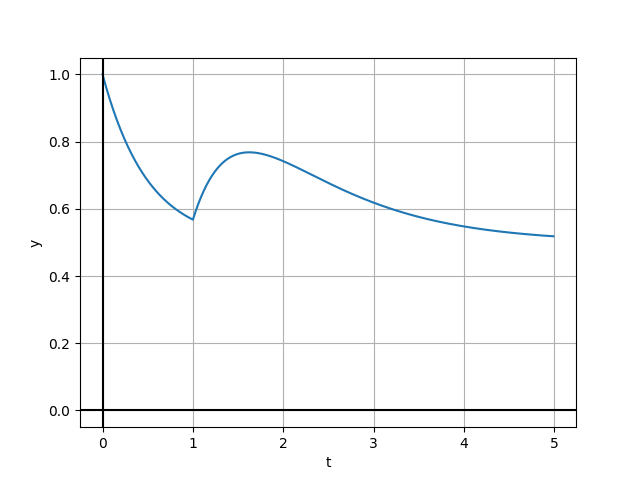
\includegraphics[width=0.9\textwidth]{media/graph.png}
        \end{center}
    \end{solution}
\end{document}
